\section{Movimento Oscilatório}
\subsection{Conteúdo Importante}
\subsubsection{Movimento Harmónico Simples}

Neste capítulo, consideramos sistemas que têm um movimento que se repete ao longo do tempo, isto é, é um movimento \textbf{periódico}. Em particular, consideramos sistemas que têm uma coordenada (e.g. $x$) que tem uma dependência sinusoidal com o tempo.

Um gráfico de $x\ vs.\ t$ para este tipo de movimento é mostrado na figura abaixo. Supondo que a partícula tem uma movimento sinusoidal periódico no eixo dos $x$, e o seu movimento oscila entre $x=+A$ e $x=-A$. Então, a expressão geral de $x(t)$ é dada por

\begin{equation}\label{eq:harmonic}
    x(t)=Acos(\omega t+\phi)
\end{equation}

$A$ é a \textbf{amplitude} do movimento. $\omega$ é a \textbf{frequência angular}. 

Da Equação \ref{eq:harmonic}, infere-se que quando o tempo $t$ aumenta em  $\frac{2\pi}{\omega}$, o argumento do $\cos$ aumenta em $2\pi$ e o valor para $x$ vai ser o mesmo. Portanto, o movimento repete-se após um intervalo de tempo $\frac{2\pi}{\omega}$, denotado por $T$, como o período do movimento.

\begin{figure}[h!]
    \centering
    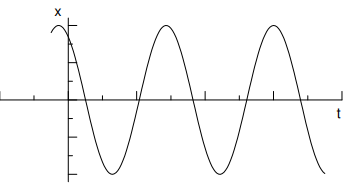
\includegraphics[width=0.5\textwidth]{10/fig/harmonic.png}
    \caption{Gráfico posição-tempo para movimento harmónico simples.}
\end{figure}

O número de oscilações por tempo é dado por $f=\frac{1}{T}$, chamada a \textbf{frequência} do movimento:

\begin{equation}
    T=\frac{2\pi}{\omega} \qquad f=\frac{1}{T}=\frac{\omega}{2\pi}
\end{equation}

Reagrupando os termos, temos uma fórmula para $\omega$ em termos de $f$ ou $T$:

\begin{equation}
    \omega=2\pi f=\frac{2\pi}{T}
\end{equation}

De $x(t)$, podemos obter a velocidade e a aceleração da partícula:

\begin{equation}
    v(t)=\frac{dx}{dt}=-\omega A\sin(\omega t+\phi)
\end{equation}

\begin{equation}\label{eq:harm-acc}
    a(t)=\frac{dv}{dt}=-\omega^2A\cos(\omega t + \phi)
\end{equation}

Note-se que os valores máximos de $v$ e $a$ são:

\begin{equation}
    v_{max}=\omega A \qquad a_{max}=\omega^2A
\end{equation}

A partícula atinge $v_{max}$ no \emph{meio} da oscilação (quando $x=0$). A magnitude da aceleração é maior nos extremos da oscilação (quando $x=\pm A$).

Comparando a Equação \ref{eq:harmonic} e a Equação \ref{eq:harm-acc}, temos:

\begin{equation}\label{eq:osc-massa-pos-1}
    \frac{d^2x}{dt^2}=-\omega^2x
\end{equation}

que é igual a $a(t)=-\omega^2x(t)$. É possível mostrar que a seguinte relação entre a velocidade $|v(t)|$ e a coordenada $x(t)$:

\begin{equation}
    |v(t)|=\omega A|\sin(\omega t+\phi)|=
    \omega A \sqrt{1-(\cos(\omega t + \phi)^2)}=\omega A\sqrt{1-(\frac{x(t)}{A})^2}.
\end{equation}

\subsubsection{Massa Ligada a uma Mola}
Supondo que uma massa $m$ está ligada à extremidade de uma mola com constante de força $k$ e desliza sobre uma superfície sem atrito.

\begin{figure}[h!]
    \centering
    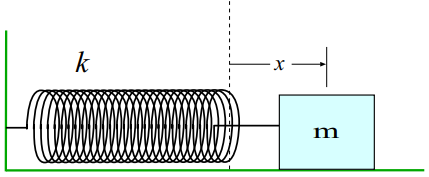
\includegraphics[width=0.5\textwidth]{10/fig/sistema.png}
    \caption{Massa $m$ ligada a uma mola horizontal com constande de força $k$; $m$ desliza sobre uma superfície sem atrito.}
\end{figure}

Então, se medirmos a coordenada $x$ da massa desde o ponto onde essa mesma massa estaria se a mola estivesse em equilíbrio, a Segunda Lei de Newton diz que:

\begin{equation*}\label{eq:osc-pos-massa-2}
    F_x=-kx=ma_x=m\frac{d^2x}{dt^2}
\end{equation*}

tendo então

\begin{equation}
    \frac{d^2x}{dt^2}=-\frac{k}{m}x
\end{equation}

Comparando a Equação \ref{eq:osc-pos-massa-2} e \ref{eq:osc-pos-massa-1}, podemos identificar $\omega^2$ como $\frac{k}{m}$ para que se tenha

\begin{equation}
    \omega=\sqrt{\frac{k}{m}}
\end{equation}

Da frequência angular $\omega$ podemos descobrir o tempo $T$ e a frequência $f$ do movimento:

\begin{equation}
    T=\frac{2\pi}{\omega}=2\pi\sqrt{\frac{m}{k}} \qquad f=\frac{1}{T}=\frac{1}{2\pi}\sqrt{\frac{k}{m}}
\end{equation}

Atente-se que $\omega$ (e, por consequência, $T$ e $f$) não dependem da amplitude $A$ do movimento da massa. Na realidade, se o movimento da massa for muito grande, então a mola não obedecerá a Lei de Hooke, mas desde que as oscilações sejam "pequenas", o periodo é o mesmo para todas as amplitudes.

\subsubsection{Energia e Oscilador Harmónico Simples}

Para o sistema massa-mola, a energia cinética é dada por

\begin{equation}\label{eq:osc-k}
    K=\frac{1}{2}mv^2=\frac{1}{2}m\omega^2A^2(\sin(\omega t + \phi)^2)
\end{equation}

e a energia potencial é

\begin{equation}
    U=\frac{1}{2}kx^2=\frac{1}{2}kA^2(\cos(\omega t +\phi)^2)
\end{equation}

Usando $\omega^2=\frac{k}{m}$ na Equação \ref{eq:osc-k}, temos que a energia total do sistema é:

\begin{equation}
    E=K+U=\frac{1}{2}kA^2[(\sin(\omega t + \phi))^2+(\cos(\omega t + \phi)^2)]
\end{equation}

Da entidade trigonométrica $\sin^2\theta+\cos^2\theta=1$, temos

\begin{equation}
    E=\frac{1}{2}kA^2
\end{equation}

mostrando que a energia de um oscilador harmónico simples (como exemplificado pelo sistema massa-mola) é constante e igual à energia potencial da mola quando está estendida ao máximo (no instante de tempo em que a massa não tem movimento).

Da Equação \ref{eq:osc-k}, temos a energia cinética em função do tempo:

\begin{equation*}
    K=\frac{1}{2}mv^2=\frac{1}{2}m\omega^2A^2\sin^2(\omega t +\phi)
\end{equation*}

O valor máximo da energia cinética é $\frac{1}{2}m\omega^2A^2$, que ocorre quando $x=0$. Visto que podemos decidir o "ponto zero" da energia potencial, temos que $U(x)=0$ em $x=0$. Então, a energia total do sistema é igual ao valor máximo da energia cinética:

\begin{equation*}
    E=\frac{1}{2}m\omega^2A^2
\end{equation*}

Usando as expressões acima, temos a energia potencial do sistema:

$$
\begin{aligned}
    U&=E-K \\
    &=\frac{1}{2}m\omega^2A^2-\frac{1}{2}m\omega^2A^2\sin^2(\omega t +\phi)=\frac{1}{2}m\omega^2A^2(1-\sin^2(\omega t + \phi)) \\
    &=\frac{1}{2}m\omega^2A^2\cos^2(\omega t + \phi) \\
    &=\frac{1}{2}m\omega^2x^2
\end{aligned}
$$

Para o sistema massa-mola, $U$ é dada por $\frac{1}{2}kx^2$, que nos dá a relação $m\omega^2=k$ ou $\omega=\sqrt{\frac{k}{m}}$, encontrada anteriormente. Usando a relação $v_{max}=\omega A$, a energia potencial pode ser escrita como

\begin{equation}
    U(x)=\frac{1}{2}m\omega^2x^2=\frac{1}{2}\frac{mv^2_{max}}{A^2}x^2
\end{equation}

\subsubsection{Relação com o Movimento Circular Uniforme}

Existe uma correspondência entre o movimento harmónico simples e o movimento circular uniforme, ilustrado na figura abaixo.

\begin{figure}[h!]
    \centering
    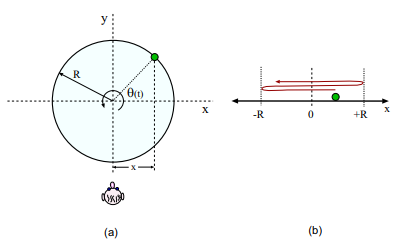
\includegraphics[width=0.5\textwidth]{10/fig/mhs-mcu.png}
    \caption{Massa $m$ ligada a uma mola horizontal com constande de força $k$; $m$ desliza sobre uma superfície sem atrito.}
\end{figure}

Na figura (a), uma massa move-se num caminho circular horizontal com movimento circular uniforme de raio $R$. A sua velocidade angular é $\omega$, logo a sua localização é dada por

\begin{equation*}
    \theta(t)=\omega t + \phi
\end{equation*}

Na figura (b) está representado o movimento da massa como se fosse vista por alguém que estivesse na direção $+y$ ao nível do disco onde a massa roda. Tal observador apenas vê mudança na coordenada $x$. Visto que $x=Rcos\theta$, a coordenada observada é

\begin{equation*}
    x(t)=Rcos(\theta(t))=Rcos(\omega t + \phi)
\end{equation*}

\subsubsection{Pêndulo}

\begin{figure}[h!]
    \centering
    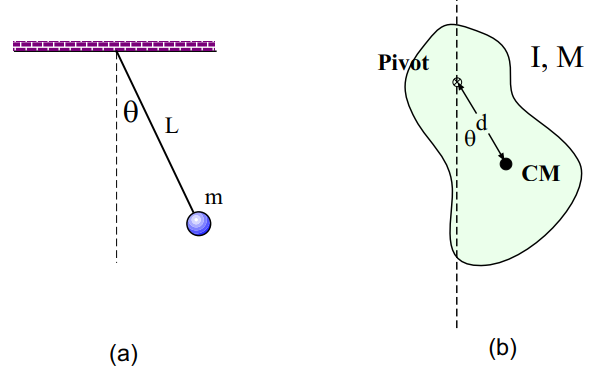
\includegraphics[width=0.5\textwidth]{10/fig/pendulos.png}
    \caption{(a) Pêndulo simples. (b) Pêndulo físico.}
\end{figure}

Abordamos, primeiro, o \textbf{pêndulo simples}, que tem uma massa $m$ suspensa por uma corda de comprimento $L$ cuja massa pode ser ignorada. A massa é colocada em movimento num plano vertical. É possível mostrar que se $\theta$ é o ângulo que a corda faz com a vertical, obedece à seguinte equação:

\begin{equation}
    \frac{d^2\theta}{dt^2}=-\frac{g}{L}\sin\theta
\end{equation}

Quando se restringe $\theta$ a valores "pequenos", podemos usar a aproximação $\sin \theta \approx \theta$, que é verdade se $\theta$ for medido em radianos. Nesse caso, a equação acima é reescrita como

\begin{equation}
    \frac{d^2\theta}{dt^2}=-\frac{g}{L}\theta
\end{equation}

Comparando a equação acima com a Equação \ref{eq:osc-massa-pos-1}, podemos identificar a frequência angular do movimento:

\begin{equation}
    \omega=\sqrt{\frac{g}{L}}
\end{equation}

\begin{equation}
    T=\frac{2\pi}{\omega} \qquad f=\frac{1}{T}=\frac{1}{2\pi}\sqrt{\frac{g}{L}}
\end{equation}

Das equações acima, infere-se que não têm qualquer dependência com a massa suspensa na corda ou com a amplitude do balanço, desde que o ângulo $\theta$ seja pequeno.

\begin{equation}
    \theta(t)=\theta_{max}\cos(\omega t + \phi)
\end{equation}

Uma generalização do pêndulo simples é a de um corpo rígido que está livre para girar num plano em torno de um eixo sem atrito. Tal sistema é conhecido como um \textbf{pêndulo físico}.

Supondo que olhamos em direção a linha uma que une o eixo ao centro de massa do objeto. Se $\theta$ for o ângulo que esta linha faz com a vertical, e se de novo for usada a aproximação $\sin\theta \approx \theta$, é possível mostrar que obedece à seguinte equação

\begin{equation}
    \frac{d^2\theta}{dt^2}=-\frac{Mgd}{I}\theta
\end{equation}

onde $d$ é a distância entre o eixo e oc entro de massa, $M$ é a massa do objeto e $I$ é o momento de inércia do objeto sobre o eixo dado.

O período $T$ é dado por:

\begin{equation}
    T=\frac{2\pi}{\omega}=2\pi\sqrt{\frac{I}{Mgd}}
\end{equation}